%*******************************************************************************************
% File ini merupakan file template LaTEX untuk penulisan Disertasi pada Universitas Gunadarma Tahun 2018
%% Programmer  : Robby Kurniawan Harahap
%% E-mail  : robby_kurniawan@staff.gunadarma.ac.id
%% Pembuatan program template makalah ini dibuat dengan menggunakan :
%% Linux Opensuse Leap 42.3
%% texstudio versi 2.12.10 dan kile
%% TeX Live 2016/TeX Live for SUSE Linux
%% acrobat reader atau okular

%*******************************************************************************************

%berikut langkah-langkah untuk mendapatkan hasil akhir Disertasi
%================================================================
%Untuk pengguna texstudio (Linux dan Windows) :
% buka template, MainTemplateDisertasi.tex
% run compile atau tekan tombol f9 pada keyboard untuk mendapatkan hasil

%Untuk pengguna texmaker (Linux dan Windows):
% buka template, MainTemplateDisertasi.tex
% run compile untuk mendapatkan hasil

%Untuk pengguna kile:
% buka template, MainTemplateDisertasi.tex
% run compile PDFLatex untuk mendapatkan hasil

%berikut ini langkah-langkah untuk mendapatkan hasil akhir disertasi

%==============================================================
% Untuk platform Windows, berikut software yang diperlukan :
% 1. MiKTeX (Latex versi Windows). Dapat didownload dari situs http://miktex.org/
% 2. WinEdt (dapat didownload dari http://www.winedt.com
% 3. ghostscript
% 4. gimp untuk mengedit gambar
% 5. Adobe reader atau foxit reader

%==============================================================
% 
%  berikut ini langkah-langkah untuk mendapatkan hasil akhir disertasi menggunakan  WinEdt :
%  tekan tombol Latex
%  tekan tombol bibtex
%  tekan tombol makeindex
%  tekan tombol Latex
%  tekan tombol Latex
%  tekan tombol Pdf Latex/Pdf Texify
%=======================================================================================================
% jika terjadi masalah dalam penulisan silahkan hubungi programmer 
%% E-mail  : robby_kurniawan@staff.gunadarma.ac.id

\documentclass[a4paper,12pt,oneside]{disertasi}

\usepackage[indonesian]{babel}
\usepackage[T1]{fontenc}
\usepackage[latin1]{inputenc}
\setcounter{secnumdepth}{3}
\setcounter{tocdepth}{3}
\usepackage{array}
\usepackage{graphicx}
\usepackage{setspace}
\usepackage{multind}
\usepackage{rotating} %for rotate/sideway text
\usepackage{subfig} %for make floating sub-figure
\usepackage{natbib}
\usepackage[linesnumbered,ruled]{algorithm2e}
\usepackage{float}
 \usepackage{lscape}
 \usepackage{pseudocode}
 \usepackage{listings}
 \usepackage{url}
\usepackage{lipsum}
\usepackage{fancyhdr}
\usepackage[linktocpage]{hyperref}
\usepackage{supertabular}
\usepackage{adjustbox}
\usepackage{multicol}
\usepackage{multirow}
\usepackage{tabularx}
\usepackage{textcomp}
\usepackage{xcolor}
\usepackage{verbatim}
\usepackage{threeparttable}
\usepackage{longtable}
\usepackage{enumitem}
\usepackage[acronym,nomain,nonumberlist]{glossaries}
\usepackage[acronym]{glossaries}
\usepackage{amsmath,amssymb,amsfonts}
\usepackage{color,soul}
\usepackage{flexisym}
\usepackage{gensymb}
\usepackage{url}
\usepackage[font=small,labelfont=bf]{caption}
\usepackage{pifont}

%\makeindex{subject}
\centerchapter
\makeatletter
\onehalfspacing
%\doublespacing
\makeatother
\parindent 3.0em
%===================================================================
\setlength{\textwidth}{15.0cm}
\setlength{\evensidemargin}{2.5cm} % outer/right margin
%\setlength{\topmargin}{0.3cm}      % top margin
\setlength{\footskip}{2.5cm}         % distance between text and foot
\setlength{\textheight}{\paperheight}
\addtolength{\textheight}{-\topmargin}
\addtolength{\textheight}{-\headheight}
\addtolength{\textheight}{-\headsep}
\addtolength{\textheight}{-\footskip}
\addtolength{\textheight}{-4cm}   % bottom margin
%==============================================================================
%% Bagian Pemenggalan Kata Yang Tidak Sempurna
%%%%%%%%%%%%%%%%%%%%%%%%%%%%%%%%%%%%%%%%%%%%%%%%%%%%%%%%%%%%%%%%%%%%%%%%%%%%%%%%%
% \hyphenatino{} %% kata yang dipenggal dengan tak sempurna
%==============================================================================
%% bagian ubah fungsi daftar algoritma
\renewcommand*{\listalgorithmcfname}{DAFTAR ALGORITMA}
\renewcommand*{\algorithmcfname}{Algoritma}
\renewcommand*{\algorithmautorefname}{Algoritma}
\newcommand{\abbrlabel}[1]{\makebox[3cm][l]{\textbf{#1}\ \dotfill}}
\newenvironment{abbreviations}{\begin{list}{}{\renewcommand{\makelabel}{\abbrlabel}}}{\end{list}}

\renewcommand{\headrulewidth}{2pt}

\begin{document}
\nocite{*}

%#start bagian administrasi #==================================================
% bagian muka sebelum isi, umumnya halaman administrasi, kalau tidak digunakan
% dapat diberikan tanda % didepannya

%cover
\pagestyle{empty}
\pagenumbering{roman}
\setcounter{page}{1}
\begin{center}

{\LARGE \selectfont \textbf{UNIVERSITAS GUNADARMA}}

\vspace{1em}

{\large \selectfont \textbf{FAKULTAS TEKNOLOGI INDUSTRI}}

\vspace{2em}

\begin{figure}[h]
\begin{center}
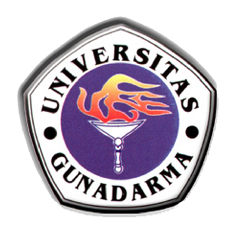
\includegraphics[scale=1.1]{LogoGundar.eps}
\end{center}
\end{figure}

\vspace{2em}

   \Large\textbf{SKRIPSI}
    
    \vspace{2em}
    \fbox{\small
        \begin{minipage}{0.9\textwidth}
            \begin{center}
                TITLE\\
                TITLE\\
                TITLE
            \end{center}
            \vspace{1em}
            \begin{tabular}{>{}ll}
                Nama         & : Nama Mahasiswa \\
                NPM          & : Nomor Pokok Mahasiswa \\
                Fakultas     & : Teknologi Industri \\
                Jurusan      & : Informatika \\
                Pembimbing   & : Nama Dosen Pembimbing dengan Gelar \\
            \end{tabular}
        \end{minipage}
    }
    
    \vspace{3em}
    {\small \selectfont \textbf{Diajukan Guna Melengkapi Sebagian Syarat}}\\
    {\small \selectfont \textbf{Dalam Mencapai Gelar Sarjana Strata Satu (S1)}}\\
    
    
    \vspace{1em}
    {\small \selectfont \textbf{JAKARTA}}\\
    {\small \selectfont \textbf{2023}}
\end{center}


% \newpage
\addcontentsline{toc}{chapter}{HALAMAN JUDUL}

\begin{center}

\begin{figure}[h]
\begin{center}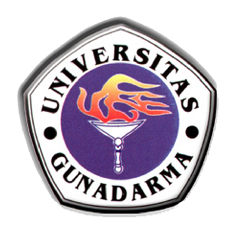
\includegraphics[%
  scale=1.1]{LogoGundar.eps}\end{center}
\end{figure}

\vspace{1.0cm}


 {\fontsize{16.5}{48} \selectfont \textbf{DETEKSI MULTI-LABEL UNTUK PENYAKIT}}\\
 {\fontsize{16.5}{48} \selectfont \textbf{MATA TIPE UMUM DAN TIPE LANGKA}}\\
  {\fontsize{16.5}{48} \selectfont \textbf{MENGGUNAKAN MULTI-MODALITAS DAN SEMANTIC DICTIONARY}}
  
 % {\fontsize{16.5}{48} \selectfont \textbf{Judul Disertasi baris 1}}\\
 % {\fontsize{16.5}{48} \selectfont \textbf{Judul Disertasi baris 2}}\\
 % {\fontsize{16.5}{48} \selectfont \textbf{Judul Disertasi baris 3}}\\
%\vfill
\vspace{1.5cm}

{\large DISERTASI}

\vspace{0.5cm}

\begin{small}Untuk Memenuhi Salah Satu Syarat Meraih Gelar Doktor Teknologi Informasi di bawah\\
 Pimpinan Rektor Universitas Gunadarma Profesor Doktor E.S. Margianti, SE, MM\\\end{small}

\vspace{0.5cm}

\begin{small}Dipertahankan dalam Sidang Terbuka Senat Universitas Gunadarma\\
Pada Hari Rabu, 3 April 2024 \\ \end{small}



\vspace{1.5cm}

{\large \underline{\textbf{{ANNEKE ANNASSIA PUTRI SISWADI}}}\\

 \vspace{0.1cm}99219002}

%\vfill

\vspace{1cm}


{\fontsize{14}{48} \selectfont \textbf{PROGRAM DOKTOR TEKNOLOGI INFORMASI}}% \vspace{0.1cm}
% \fontsize{14}{48} \selectfont \textbf{PROGRAM PASCASARJANA}\\ % \vspace{0.1cm}

{\fontsize{14}{48} \selectfont \textbf{UNIVERSITAS GUNADARMA}} % \vspace{0.1cm}

{\fontsize{14}{48} \selectfont \textbf{2024}}




\end{center} 


%halaman lembar pengesahan, abstraksi, kata pengantar
\pagestyle{plain}
\pagenumbering{roman}
\setcounter{page}{2}%nilai halaman utk awal dari abstrak s/d ucapan terimakasih dlm romawi
\newpage %Acknowledgment
\addcontentsline{toc}{chapter}{PERNYATAAN ORIGINALITAS DAN PUBLIKASI }
\begin{center}
\begin{large}\textbf{PERNYATAAN ORIGINALITAS DAN PUBLIKASI}\\\end{large}
\end{center}
\vspace{1cm}


Saya yang bertanda tangan di bawah ini:

\begin{flushleft}
\begin{tabbing}
 \hspace{4cm}\=\kill
  Nama\>: Nama mahasiswa\\
  NPM\>: 11111111 \\
 Judul Skripsi\>: \textbf{JUDUL LINE 1} \\
\> ${}$\hspace{0.65em}\textbf{JUDUL LINE 2} \\

Tanggal Sidang \>: 3 April 2024\\
Tanggal Lulus \>: 3 April 2024 \\
\end{tabbing}

\end{flushleft}

Menyatakan bahwa tulisan ini adalah merupakan hasil karya saya sendiri dan dapat dipublikasikan sepenuhnya oleh Universitas Gunadarma. Segala kutipan dalam bentuk apapun telah mengikuti kaidah dan etika yang berlaku. Semua hak cipta dari logo serta produk yang disebut dalam buku ini adalah milik masing-masing pemegang haknya, kecuali disebutkan lain. Mengenai isi dan  tulisan  adalah merupakan tanggung jawab Penulis, bukan  Universitas Gunadarma. 

Demikian pernyataan ini dibuat dengan sebenarnya dan dengan penuh kesadaran.
\vspace{0.5 cm}
\begin{flushleft}

Depok, 3 April 2024 %% Tahun penulisan

\vspace{1.5 cm}
(NAMA MAHASISWA)
\end{flushleft} 
\newpage

\addcontentsline{toc}{chapter}{LEMBAR PENGESAHAN}

\begin{center}
    \begin{large}\textbf{ LEMBAR PENGESAHAN} \end{large} \\[2cm]

    \textbf{\normalsize KOMISI PEMBIMBING} \\[0.5cm]

    \begin{table}[H]
        \centering
        \begin{tabular}{|c|c|c|}
        \hline
        \textbf{NO} & \textbf{NAMA} & \textbf{KEDUDUKAN} \\ \hline
        1. & \rule{6cm}{0.15mm} & Ketua \\ \hline
    \end{tabular} \\[2cm]
    \end{table}
    

    \textbf{\normalsize PANITIA UJIAN} \\[0.5cm]

    \begin{table}[H]
    \centering
    \begin{tabular}{|c|c|c|}
    \hline
        \textbf{NO} & \textbf{NAMA} & \textbf{KEDUDUKAN} \\ \hline
        1. & \rule{6cm}{0.15mm} & Ketua \\ \hline
        2. & \rule{6cm}{0.15mm} & Sekretaris \\ \hline
        3. & \rule{6cm}{0.15mm} & Anggota \\ \hline
    \end{tabular} \\[2cm]
    \end{table}

    \textbf{\normalsize Mengetahui,} \\[1cm]
    \hspace{1cm} \textbf{\normalsize Pembimbing} \hspace{3cm} \textbf{\normalsize Bagian Sidang Ujian} \\ [2cm]
    \textbf{\footnotesize (Nama Pembimbing dengan gelar)} \textbf{\footnotesize (Nama Bagian Sidang Ujian dengan gelar)} \\
\end{center}
% menggabungkan file lembar pengesahan
\newpage %Abstract
\addcontentsline{toc}{chapter}{ABSTRAK}
\begin{center}
\vspace{10mm}
\begin{large}\textbf{Abstrak}\end{large}
\end{center}

\noindent
Nama. NPM \\
JUDUL PENELITIAN. \\
Skripsi, Fakultas Teknologi Industri, Jurusan Informatika, Universitas Gunadarma, 2025. \\
Kata Kunci: Kata Kunci 1, Kata Kunci 2, Kata Kunci 3
\\
(xiv + 81 + lampiran) \\

\vspace{2mm}

\begin{singlespacing}
% Abstrak ini tidak melebihi 350 kata dan paragraf dengan ukuran 1 spasi
\lipsum[1]

\end{singlespacing}
\noindent \\
\noindent Daftar Pustaka (2013-2024)% menggabungkan file abstraksi
\newpage %Abstract
\addcontentsline{toc}{chapter}{ABSTRACT}
\begin{center}
\vspace{10mm}
\begin{large}\textbf{Abstract}\end{large}
\end{center}

\noindent
Name. NPM \\
RESEARCH TITLE. \\
Undergraduate Thesis, Informatics, Faculty of Industrial Technology, Gunadarma University, 2025. \\
Keywords: Keyword 1, Keyword 2, Keyword 3
\\
(xiv + 81 + lampiran) \\

\vspace{3mm}

\begin{singlespacing}
\lipsum[1]

\end{singlespacing}

\noindent \\

\noindent 
Reference (2013-2024)
%menggabungkan file CV atau riwayat hidup ringkas
%\include{cv}
\newpage %Acknowledgment
\addcontentsline{toc}{chapter}{KATA PENGANTAR}
\begin{center}
\begin{large}\textbf{KATA PENGANTAR}\\\end{large}
\end{center}
\vspace{5mm}
\textit{Bismillahirrohmaanirrohiim} \\
\textit{Assalamu'alaikum Warahmatullahi Wabarakatuh}

Alhamdulillahi rabbil 'aalamiin. Segala puji dan syukur hanya kepada ALLAH SWT, atas rahmat dan karunia-NYA, Penulis dapat menyelesaikan Tugas Akhir ini. Tugas akhir ini disusun sebagai salah satu syarat untuk memperoleh gelar Sarjana Komputer dari Universitas Gunadarma. Judul Tugas Akhir ini adalah "JUDUL TUGAS AKHIR". Shalawat dan salam Penulis sampaikan kepada suri teladan kita, manusia biasa dengan akhlak luar biasa, Rasulullah SAW.

Penulis menyadari bahwa dalam proses penyusunan Tugas Akhir ini, tidak terlepas dari bantuan, bimbingan, dorongan, dan doa yang tulus dari banyak pihak. Oleh karena itu, pada kesempatan yang berbahagia ini, dengan segala kerendahan dan ketulusan hati, penulis ingin mengucapkan terima kasih yang sebesar-besarnya kepada:


\begin{enumerate}
\item Prof. Dr. E.S. Margianti, S.E., MM.,  selaku Rektor Universitas Gunadarma.
\item Prof. Dr.-Ing. Adang Suhendra, SSi., SKom, MSc., selaku Dekan Fakultas Teknologi Industri Universitas Gunadarma.
\item Prof. Dr. Lintang Yuniar Banowosari, S.Kom., M.Sc., selaku Ketua Program Studi Informatika Universitas Gunadarma.
\item Dr. Edi Sukirman, SSi., MM., M.I. Kom., selaku Kepala Bagian Sidang Ujian Universitas Gunadarma.
\item Nama Dosen Pembimbing dengan Gelar, selaku Dosen Pembimbing yang telah banyak meluangkan waktu dalam membimbing, mengarahkan, memberi masukan, ilmu pengetahuan, dan koreksi dengan penuh kesabaran, sehingga tugas akhir ini menjadi lebih baik.
\item Kedua orang tua, yaitu Nama Ayah dan Nama Ibu sebagai orang tua penulis yang telah memberikan dukungan yang luar biasa beserta do'a yang tidak kunjung putus sehingga tugas akhir ini dapat selesai dengan hasil yang terbaik.
\item Seluruh rekan dan pihak yang telah membantu selama mengerjakan dan meyelesaikan tugas akhir ini.
\end{enumerate}

Akhir kata semoga tugas akhir ini bermanfaat bagi siapa saja yang mengkajinya dan dapat dikembangkan serta disempurnakan untuk menambah kemanfaatan bagi banyak orang.

\vspace{0.5 cm}

\textit{Wabillahi taufiq wal hidayah}

\textit{Wassalamu'alaikum Warahmatullahi Wabarakatuh}

% Bagian akhir dari kata pengantar

% \vspace{0.5 cm}

 %\textit{Wabillahi taufiq wal hidayah}

 %\textit{Wassalamu'alaikum Warahmatullahi Wabarakatuh}

\begin{flushleft}
Depok, 3 April 2024\\
Penulis
\vspace{1.5 cm}

(Nama Lengkap Penulis)

\end{flushleft} 
% mengabungkan file kata pengantar

%# akhir bagian administrasi # ==========================================

% #mulai membuat daftar isi, daftar gambar dan  daftar tabel # ==========
%\setcounter{page}{8} %set nilai halaman sesuai urutannya

% membuat daftar isi
\addcontentsline{toc}{chapter}{DAFTAR ISI}
\tableofcontents{}

%% membuat daftar tabel
\listoftables
\addcontentsline{toc}{chapter}{DAFTAR TABEL}

%membuat daftar gambar
\listoffigures
\addcontentsline{toc}{chapter}{DAFTAR GAMBAR}%masih masalah

% \listofalgorithms
% \addcontentsline{toc}{chapter}{DAFTAR ALGORITMA}
% \include{istilah}

\newpage %lampiran
\addcontentsline{toc}{chapter}{DAFTAR LAMPIRAN}
\begin{center}
\begin{large}\textbf{DAFTAR LAMPIRAN}\\\end{large}
\end{center}
\vspace{5mm} Lampiran 1 Daftar Gejala Penyakit Mata
.........................................................
114



% #akhir membuat daftar isi, daftar gambar dan  daftar tabel # ==========

% # mulai bagian isi # ==================================================

\newpage
\pagestyle{headings}
\pagenumbering{arabic} % jenis huruf arabic
\setcounter{page}{1} %mulai dari halaman 1

 \pagestyle{fancy}

 \fancyhead[LO,RE]{\slshape \leftmark}
\rhead{\thepage}
\cfoot{}

\chapter{PENDAHULUAN}

\section{Latar Belakang}
\label{sec:1-LatarBelakang}

Pemanggilan referensi pertama kali dengan seluruh nama author \citep*{hinton2006fast} dan pemanggilan referensi untuk selanjutnya hanya nama author pertama dan et al \citep{hinton2006fast}. Daftar pustaka masukkan di \textbf{MainTemplateDisertasi.bib}.

\begin{figure}[H]
\centerline{
\includegraphics[width=.6\textwidth]{bab1/dir_gambar/DeepSeek-Logo.png}}
\caption{Citra yang tidak sehat.}
\label{cfp_bab1}
\end{figure}

Pemanggilan label pada gambar, tabel, dan sejenisnya menggunakan Gambar \ref{cfp_bab1}. 

\section{Rumusan Masalah}
\label{sec:2-Rumusanmasalah}
Berdasarkan latar belakang yang telah disampaikan, dapat disimpulkan beberapa permasalahan yang dirumuskan sebagai berikut:

\begin{enumerate}
 \item Masalah 1
 \item Masalah 2
 \item Masalah 3
\end{enumerate}

\section{Tujuan dan Batasan Penelitian}
\subsection{Tujuan Penelitian}
\label{sec:3-TujuanPenelitian}
Tujuan dari penelitian ini dirangkum sebagai berikut:
\begin{enumerate}
    \item Tujuan satu.
    \item Tujuan dua.
    \item Tujuan tiga.
\end{enumerate}

\subsection{Batasan Penelitian}
\label{sec:3-BatasanPenelitian}
Untuk menghindari meluasnya permasalahan dalam domain yang diteliti, batasan penelitian dibuat dan diringkas dalam poin-poin berikut:
\begin{enumerate}
    \item Batasan 1.
    \item Batasan 2. 
    \item Batasan 3.
\end{enumerate}

\section{Sistematika Penulisan}
 %Bab 1

\chapter{TINJAUAN PUSTAKA}
\label{cha:2-TelaahPustaka}


Contoh penggunaan dan pemanggilan Tabel \ref{tab:dataset}.

\begin{table}[H]
    
    \captionsetup{justification=centering}
	\caption{Result of localization for each dataset (in number of images)}
	\label{tab:dataset}
    \begin{adjustbox}{width=1\textwidth}
    
    \begin{tabular}{|l|c|c|c|c|c|c|c|c|}
    \hline
    
    \multirow{2}{*}{ Dataset} & \multicolumn{2}{c|}{With Outliers in 4m acc} & \multicolumn{2}{c|}{Without Outliers in 4m acc} & \multicolumn{3}{c|}{With Outliers in 1m acc} & \multicolumn{1}{c|}{Without Outliers in 1m acc}                     \\ \cline{2-9}
      & Localized      & Unlocalized & Localized         & Unlocalized & Localized      & Unlocalized & Localized         & Unlocalized \\ \hline
      
         Arc de Triomphe & 111  &  29  &  111  &  28  &  103  &  37  &  103  &  36  \\
    Barcelona       & 184  &  16  &  184  &  11  &  156  &  44  &  156  &  39  \\
    Cambridge       & 87  &  13  &  87  &  13  &  81  &  19  &  81  &  19  \\
    CERN            & 74  &  26  &  74  &  19  &  65  &  35  &  65  &  28  \\
    Chicago         & 136  &  14  &  136  &  12  &  121  &  29  &  121  &  27  \\ 
    Dubai           & 87  &  13  &  87  &  9  &  74  &  26  &  74  &  22  \\ 
    Havana          & 95  &  5  &  95  &  5  &  89  &  11  &  89  &  11  \\ 
    Indonesia       & 63  &  27  &  63  &  11  &  52  &  38  &  52  &  22  \\
    Kitakyushu      & 90  &  10  &  90  &  8  &  76  &  24  &  76  &  22  \\
    Marina Bay      & 205  &  15  &  205  &  13  &  178  &  42  &  178  &  40  \\ 
    Marrakesh       & 97  &  3  &  97  &  3  &  88  &  12  &  88  &  12  \\
    Moscow          & 98  &  2  &  98  &  2  &  90  &  10  &  90  &  10  \\
    Munich          & 90  &  10  &  90  &  8  &  79  &  21  &  79  &  19  \\
    Oslo            & 92  &  8  &  92  &  7  &  83  &  17  &  83  &  16  \\
    Paris           & 35  &  65  &  35  &  41  &  30  &  70  &  30  &  46  \\ 
    Qatar           & 183  &  17  &  183  &  11  &  162  &  38  &  162  &  32  \\
    Shanghai        & 142  &  8  &  142  &  6  &  130  &  20  &  130  &  18  \\
    Sydney          & 92  &  8  &  92  &  8  &  82  &  18  &  82  &  18  \\
    Syria           & 94  &  6  &  94  &  5  &  87  &  13  &  87  &  12  \\
    Vienna          & 83  &  17  &  83  &  14  &  75  &  25  &  75  &  22  \\ \hline
    Total           & 2138 & 312 & 2138 & 234 & 1901 & 549  & 1901 & 471 \\ \hline
 
    \end{tabular}
    \end{adjustbox}
\end{table}
 %Bab 2

\chapter{METODE PENELITIAN} %Bab 3

\chapter{HASIL DAN PEMBAHASAN}
\section{Implementasi} %Bab 4

\chapter{PENUTUP}
\section{Kesimpulan}

\section{Saran}
 %Bab 5
\newpage
% diatas menunjukkan SubDir/nama file tex, bisa ditambah/dikurang sesuai kebutuhan

% # akhir bagian isi # ==================================================

% # mulai bagian Daftar Pustaka # ============================================
\thispagestyle{empty}
\renewcommand\bibname{DAFTAR PUSTAKA}


\addcontentsline{toc}{chapter}{DAFTAR PUSTAKA} %memasukkan daftar pustaka di daftar isi
%\addtocontents{toc}{\contentsline {chapter}{\numberline {}{DAFTAR PUSTAKA}}{}}
%\Urlmuskip=0mu plus 1mu\relax
\bibliographystyle{agsm}
\bibliography{MainTemplateDisertasi} %file menyimpan bibtex

% # akhir bagian referensi # ============================================

\newpage
\pagestyle{plain}
\thispagestyle{empty}
\newpage %lampiran
\addcontentsline{toc}{chapter}{LAMPIRAN}
\singlespacing
\begin{center}
\begin{large}\textbf{LAMPIRAN}\\\end{large}
\end{center}
\vspace{5mm}

\section*{Lampiran 1}
\begin{center}

\end{center}
%\printindex{subject}{INDEKS}
\thispagestyle{empty}
\end{document}
%% Finish----------------
